\subsection{Vertex+Beamspot Constraint: VX+BS}
% \subsection{Methodology}
% so they all come from the primary vertex 
%interaction. \\
Leptons produced from the \hzzfourl channel should originate from the \pp collision point---the primary vertex---since the \PH boson and both \PZ bosons decay promptly after being formed.
% TODO: Explain why electrons are not given the vertex+beamspot constraint.
The primary vertex from which the muons originate can be approximated to come from the more general \emph{beamspot}, \ie the luminous region in the $x$-$y$ plane where the \pp bunches cross.
Thus, if the muon tracks are constrained to come from their vertex of origination ($\approx$beamspot), then one should expect a more accurate measurement of muon momentum and resolution.
The updated muon kinematical variables then get propagated into a more accurate estimate of the \mH value per event.
This process of constraining muon tracks to a vertex that is compatible with the beamspot is called the \emph{vertex+beamspot constraint} (VX+BS).

The pixel upgrade in the middle of Run 2 allowed for a more collimated (more precise) \pp beamspot.
Figure~\ref{fig:BeamY_vs_Y} shows the beamspot for 2018 Run D as compared to 2016 Run G.
Both the X and Y widths of the beamspot are smaller ($X_{2018} \approx 9 \mu m$ vs $X_{2016} \approx 14 \mu m$ and $Y_{2018} \approx 7 \mu m$ vs $Y_{2016} \approx 9 \mu m$), giving a better constraint when it is used in the track reconstruction.
% Beamspot information has been investigated in order to try to understand the reason why 2018 results have a two times better results.
% In Fig.~\ref{fig:BeamY_vs_Y}, the beamspot width (Y vs X) is shown for 2016 RunG and 2018 RunD.
% On the other hand, Fig.~\ref{fig:BeamXY_vs_Lumi} shows the width X and Y as a function of lumi section.
% As can be seen, in 2018, both X and Y widths of the beamspot are smaller ($X_{2018} \approx 9 \mu m$ vs $X_{2016} \approx 14 \mu m$ and $Y_{2018} \approx 7 \mu m$ vs $Y_{2016} \approx 9 \mu m$), letting a better constraint when it is used in the track reconstruction.
%=== Beamspot width Y vs. width X.
% TODO: Cut this picture up and do it properly?
\begin{multiFigure}
    \centering
        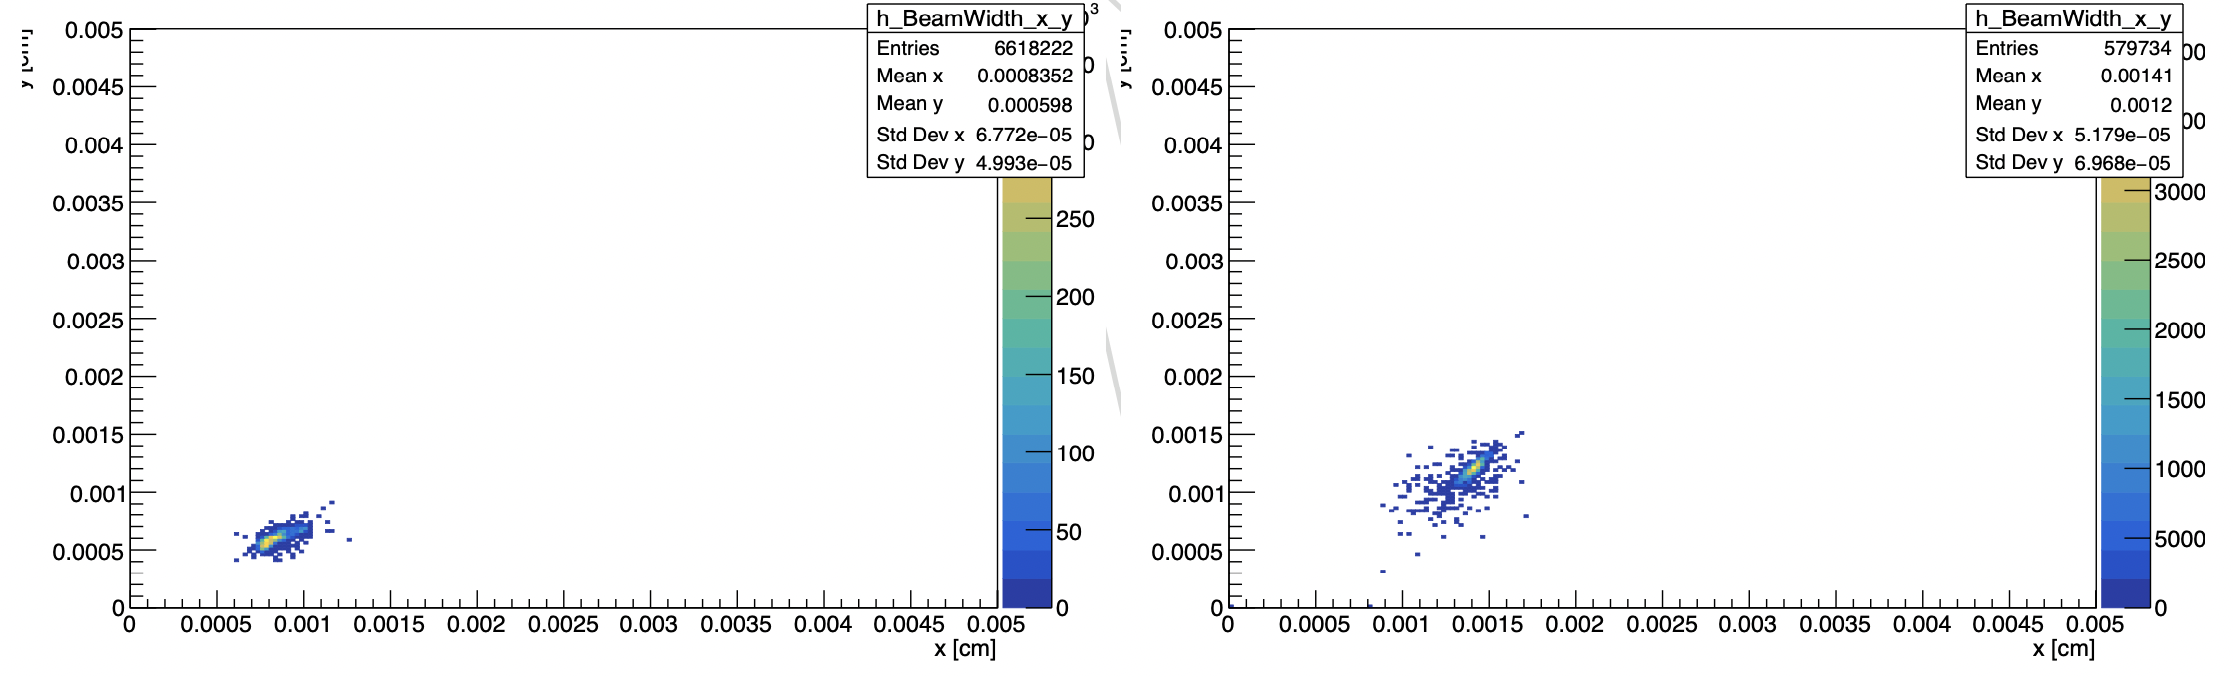
\includegraphics[width=0.96\textwidth]{figures/higgsmassmeas/vxbs/beamspot_width_2016RunG_vs_2018RunD.png}
	% \includegraphics[width=0.45\textwidth]{Figures/VXBS/2018D_VS_width_y_vs_x.pdf}
  	% \includegraphics[width=0.45\textwidth]{Figures/VXBS/2016G_VS_width_y_vs_x.pdf}
	\captionof{figure}
        [Y vs X width of beamspot for 2018 RunD \vs 2016 RunG]
        {Y vs X width of beamspot for different runs.
        \;A) 2018 Run D.
        \;B) 2016 Run G}
    \label{fig:BeamY_vs_Y}
\end{multiFigure}
Once the event is selected, the vertex+beamspot constraint is applied.

% TODO:REWORD
Muon reconstruction currently used does not take into account any information about the 
vertex production of the lepton itself. % and in the Higgs boson decay, all the leptons are prompt.
In the VX+BS approach, the four tracks from Higgs boson decay are constrained looking for a common 
vertex (VX) that must be compatible with the beamspot (BS). 
While muons information are updated after this procedure,
electrons are used only to constrain the position of the common vertex, 
leaving their kinematic information unaltered. \\
This method has been checked in DATA and in simulation, using Z boson events (60--120 GeV)
decaying into two muons: muon \pT resolution and mass resolution improves by about 5-10\%. 
This method received the green light from MuonPOG.\\ 
(Following studies within MuonPOG have been performed using UL-Summer19/20 samples.)
Figures~\ref{fig:Resolution_pT} and~\ref{fig:Resolution_eta} show muon resolution respectively 
as a function of \pT and $|\eta|$ for 2018, 2017 and 2016.
As can been seen, resolution improves by about 10$\%$ in 2018 and roughly 5$\%$ in 2016 and 2017.
\begin{multiFigure}
    \centering
        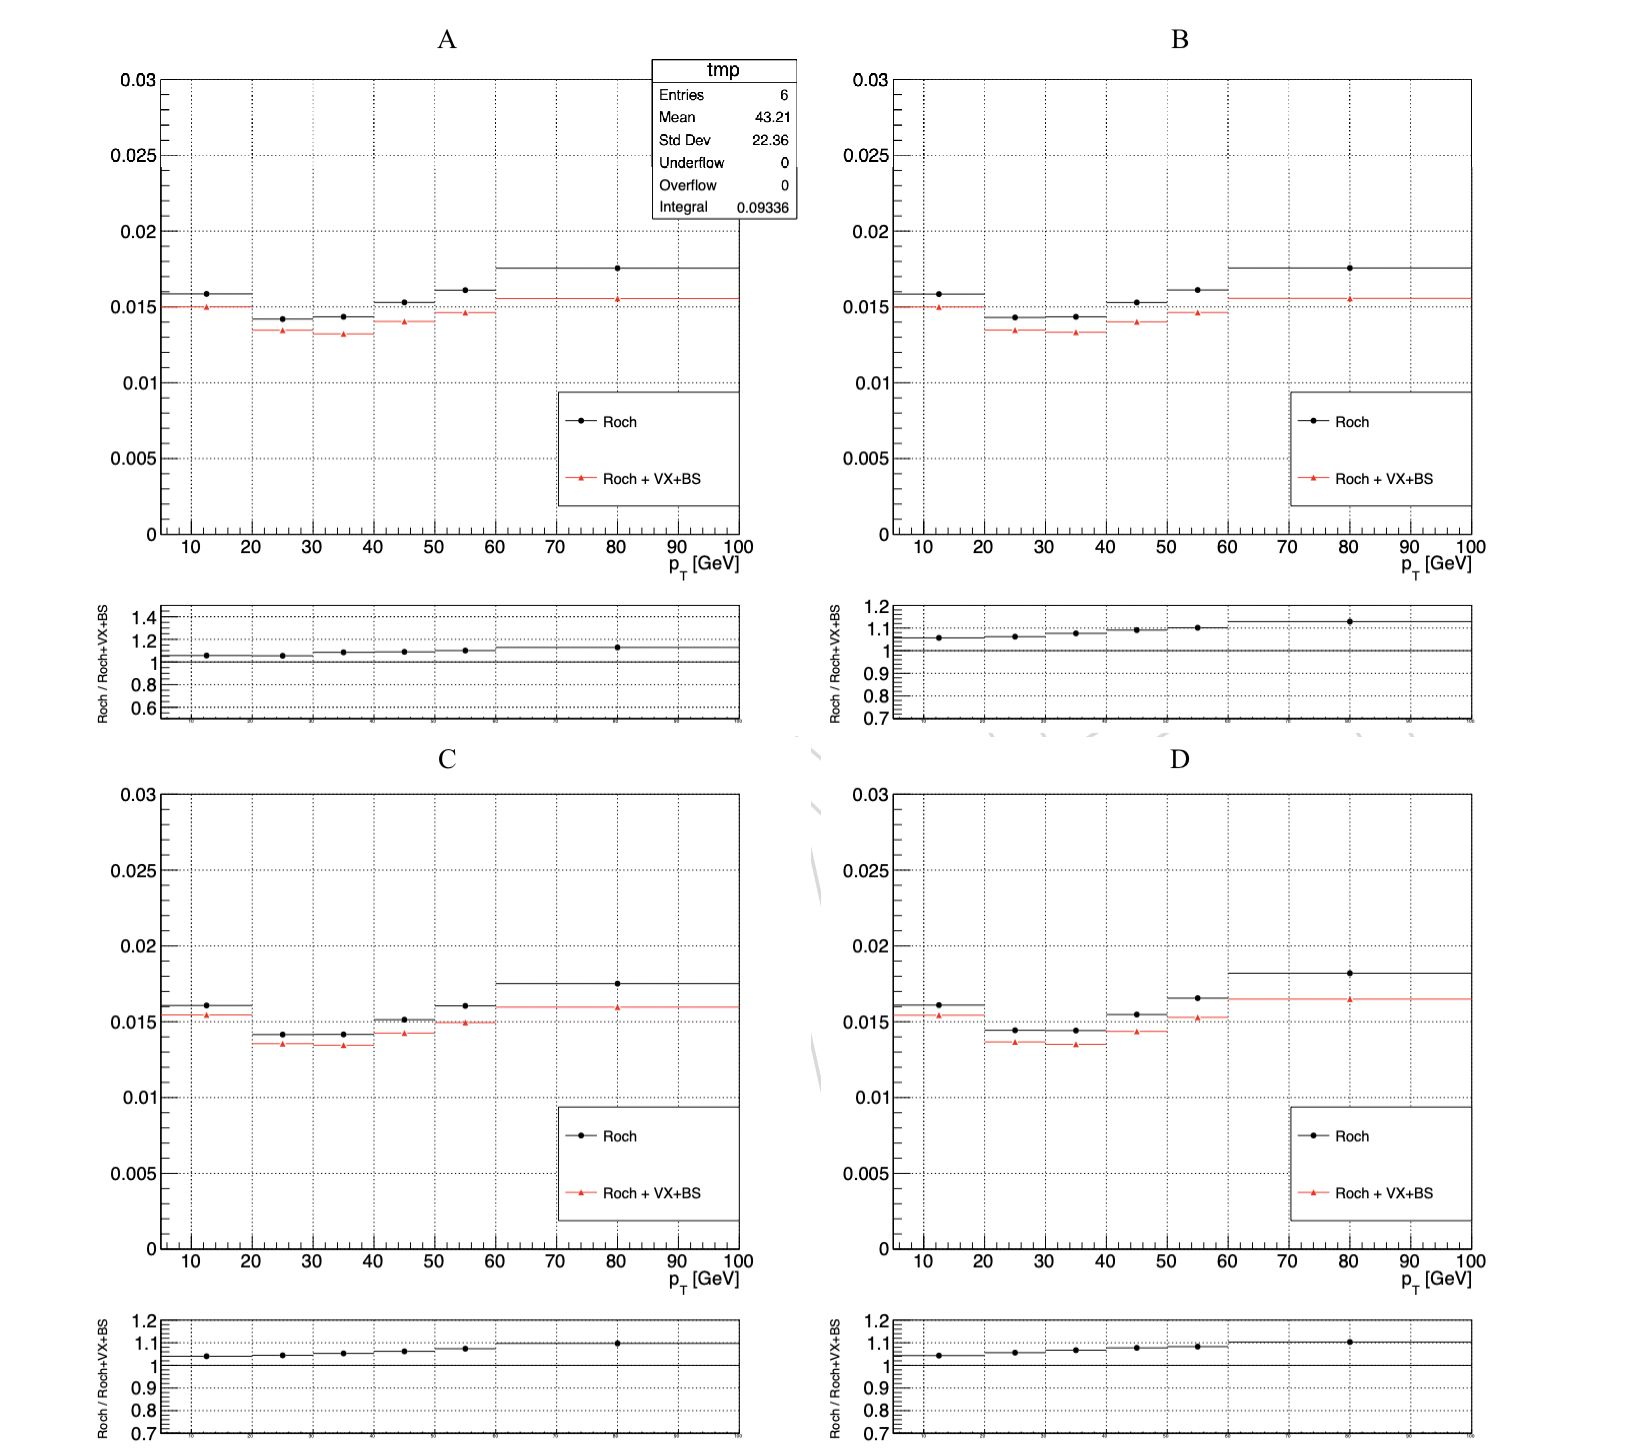
\includegraphics[width=0.96\textwidth]{figures/higgsmassmeas/vxbs/vxbs_muon_pTresol_vs_pT.png}
    \captionof{figure}
        [Muon \pT resolution as a function of \pT before and after VX+BS constraint]
        {Muon \pT resolution as a function of \pT before (black line) and after (red line) VX+BS constraint.
        \;A) 2018.
        \;B) 2017.
        \;C) 2016 post-VFP.
        \;D) 2016 pre-VFP.}
        % TODO: Use actual PDFs.
        % TODO: Split pic up properly?
\label{fig:Resolution_pT}
\end{multiFigure}
\begin{multiFigure}
    \centering
        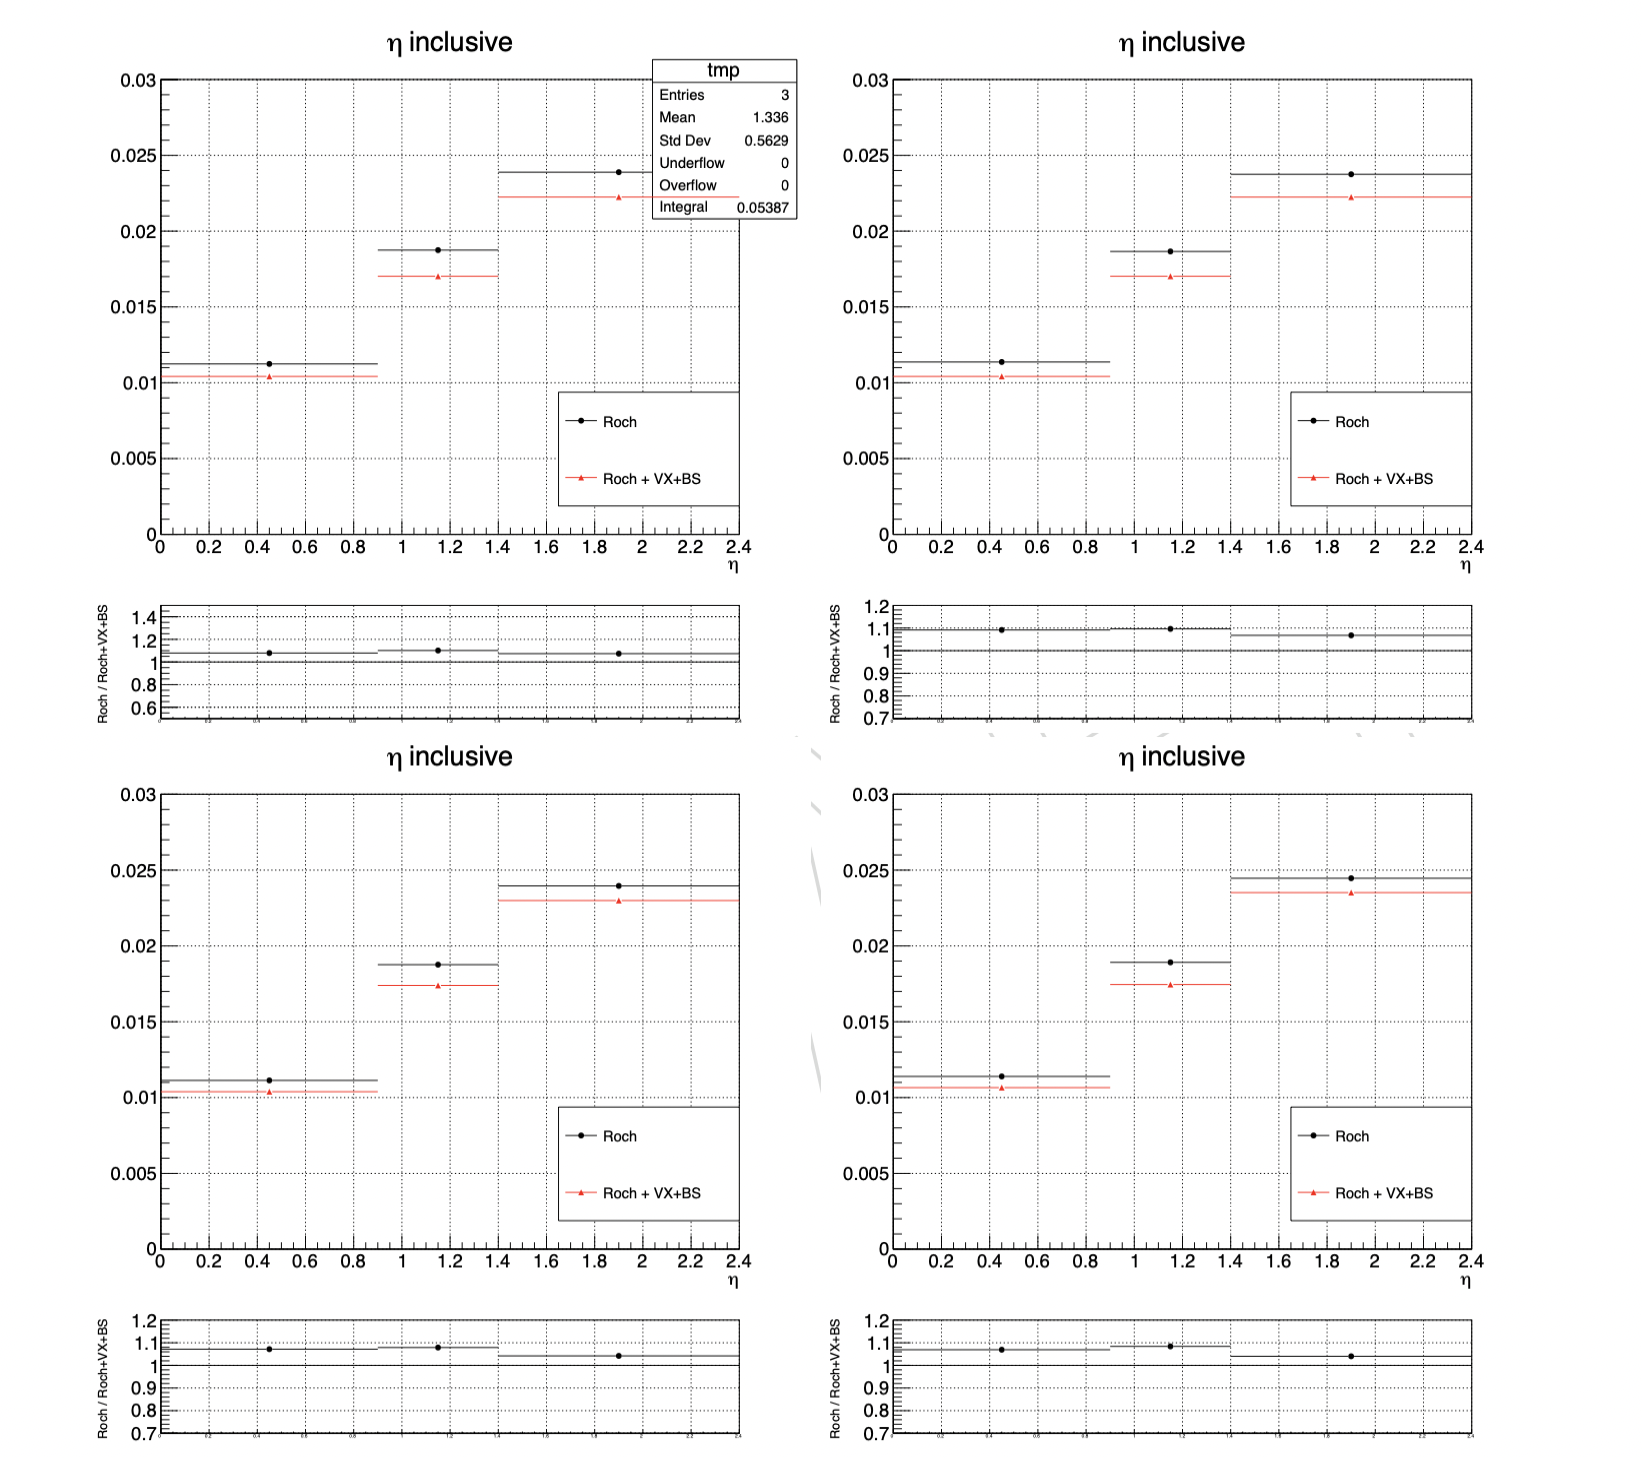
\includegraphics[width=0.96\textwidth]{figures/higgsmassmeas/vxbs/vxbs_muon_pTresol_vs_eta.png}
    \captionof{figure}
        [Muon \pT resolution as a function of \abseta before and after VX+BS constraint]
        {Muon \pT resolution as a function of \abseta before (black line) and after (red line) VX+BS constraint.
        \;A) 2018.
        \;B) 2017.
        \;C) 2016 post-VFP.
        \;D) 2016 pre-VFP.} % TODO: Use actual PDFs. Split pic up properly?
\label{fig:Resolution_eta}
\end{multiFigure}

% TODO: Find all Data-MC -> Data--MC.
Figure~\ref{UL_ZBoson_DataMC_comparison_VXBS} shows Data--MC comparison, with and without VXBS constraint.
The mean and the $\sigma$ reported on the plots are the once of the DSCB used to fit the distribution (convolved with a BW) and that simulate the detector effect.
As can been seen, the \PZ boson resolution gets improved comparably to that of the improvement of muon \pT resolution:
7\%(8\%) for 2018 DATA (MC), 5\%(4\%) for 2017, 5\%(6\%) for post-VFP and 5\%(5\%) for 2016 pre-VFP. 
\begin{multiFigure}
    \centering
        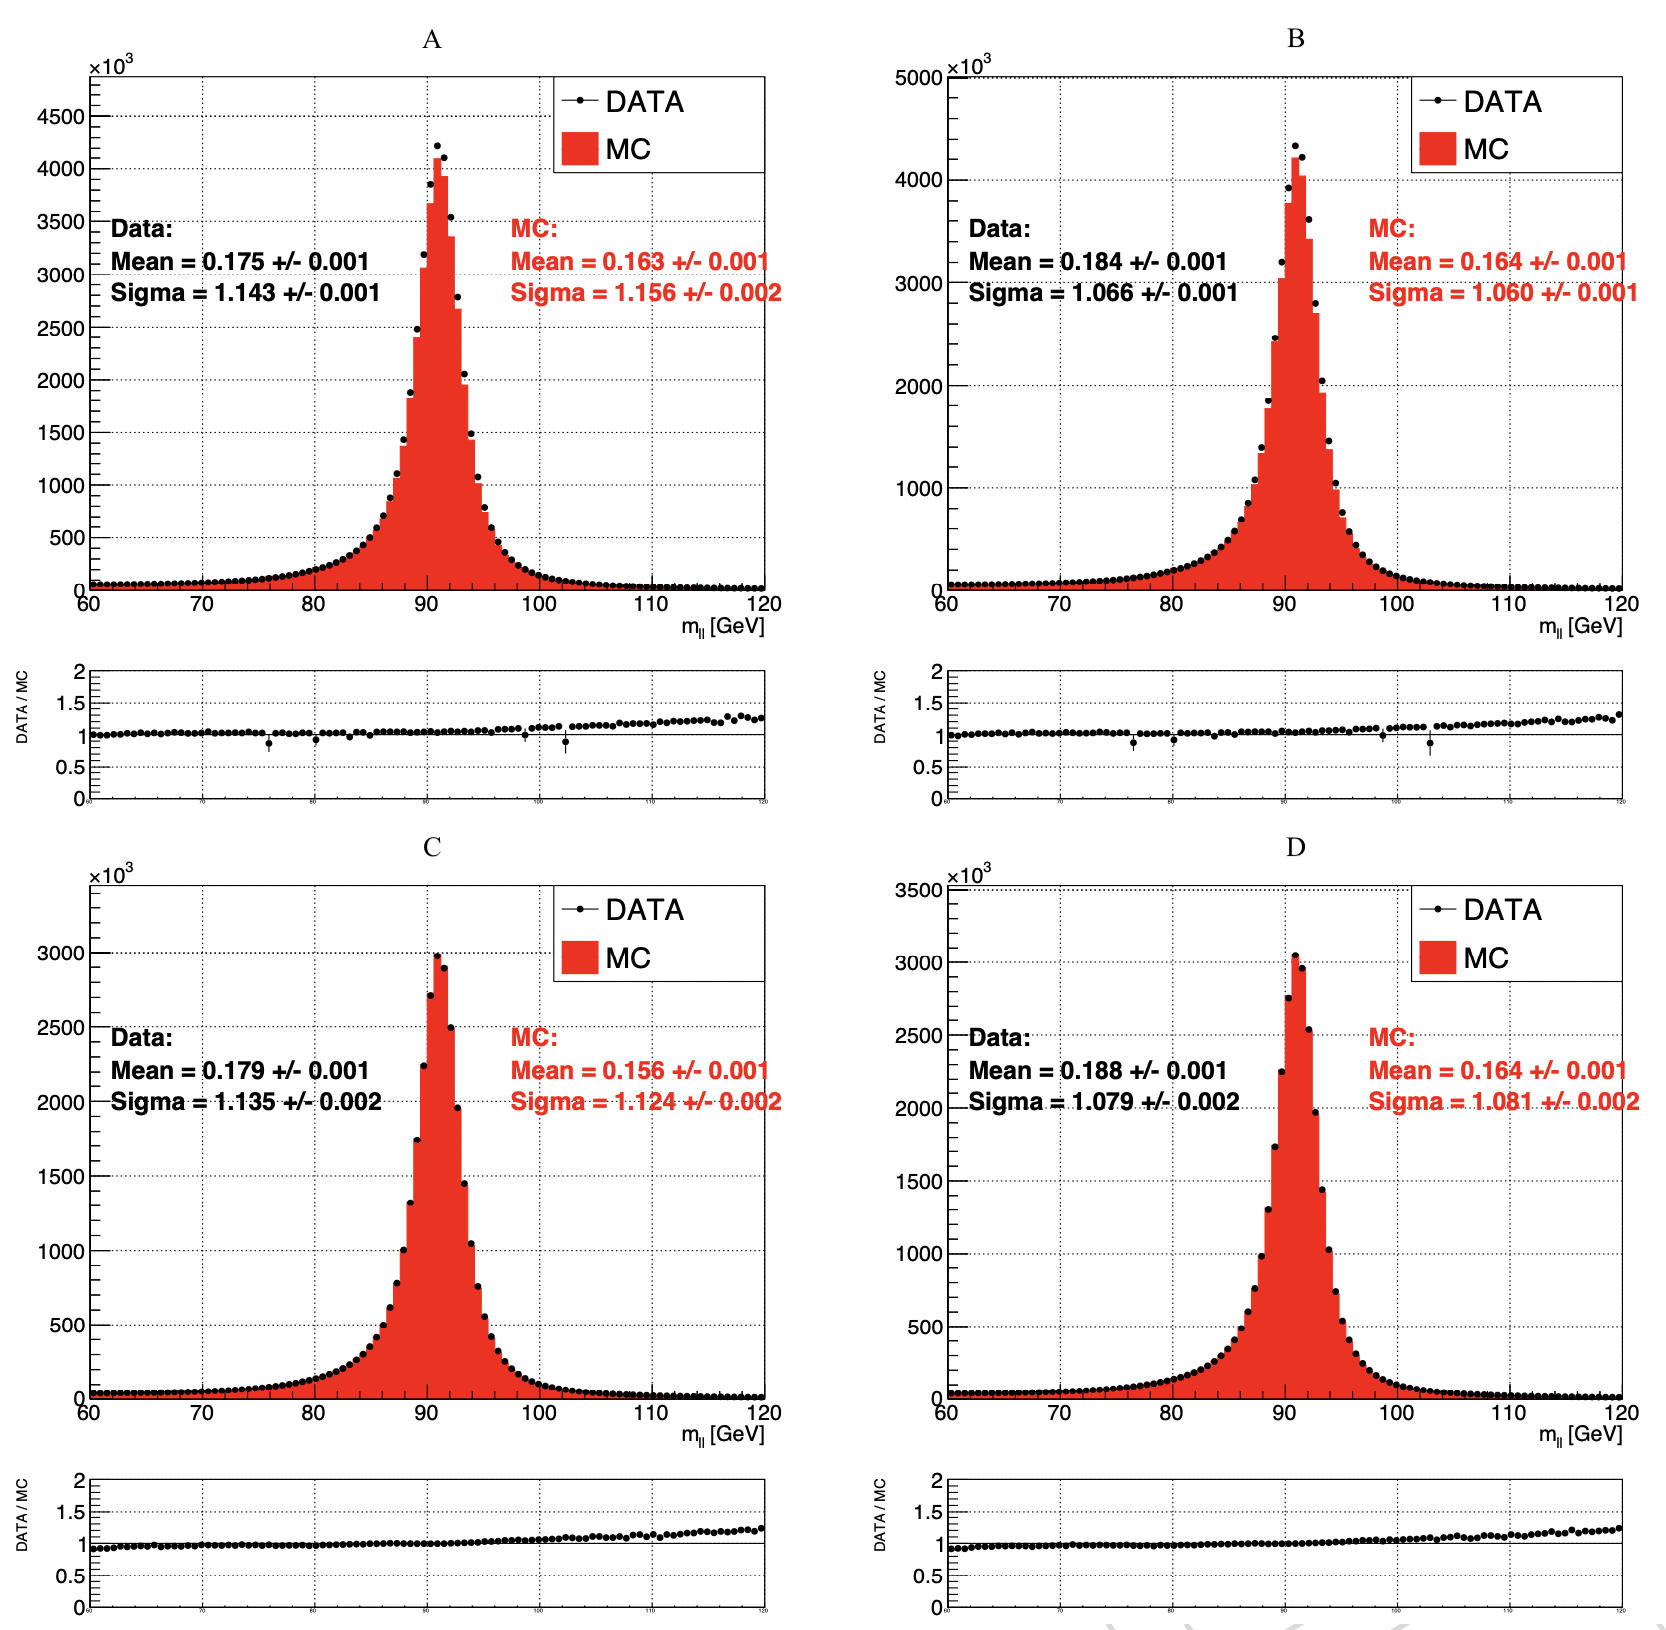
\includegraphics[width=0.96\textwidth]{figures/higgsmassmeas/vxbs/vxbs_mZdist_2017_2018.png}
	% 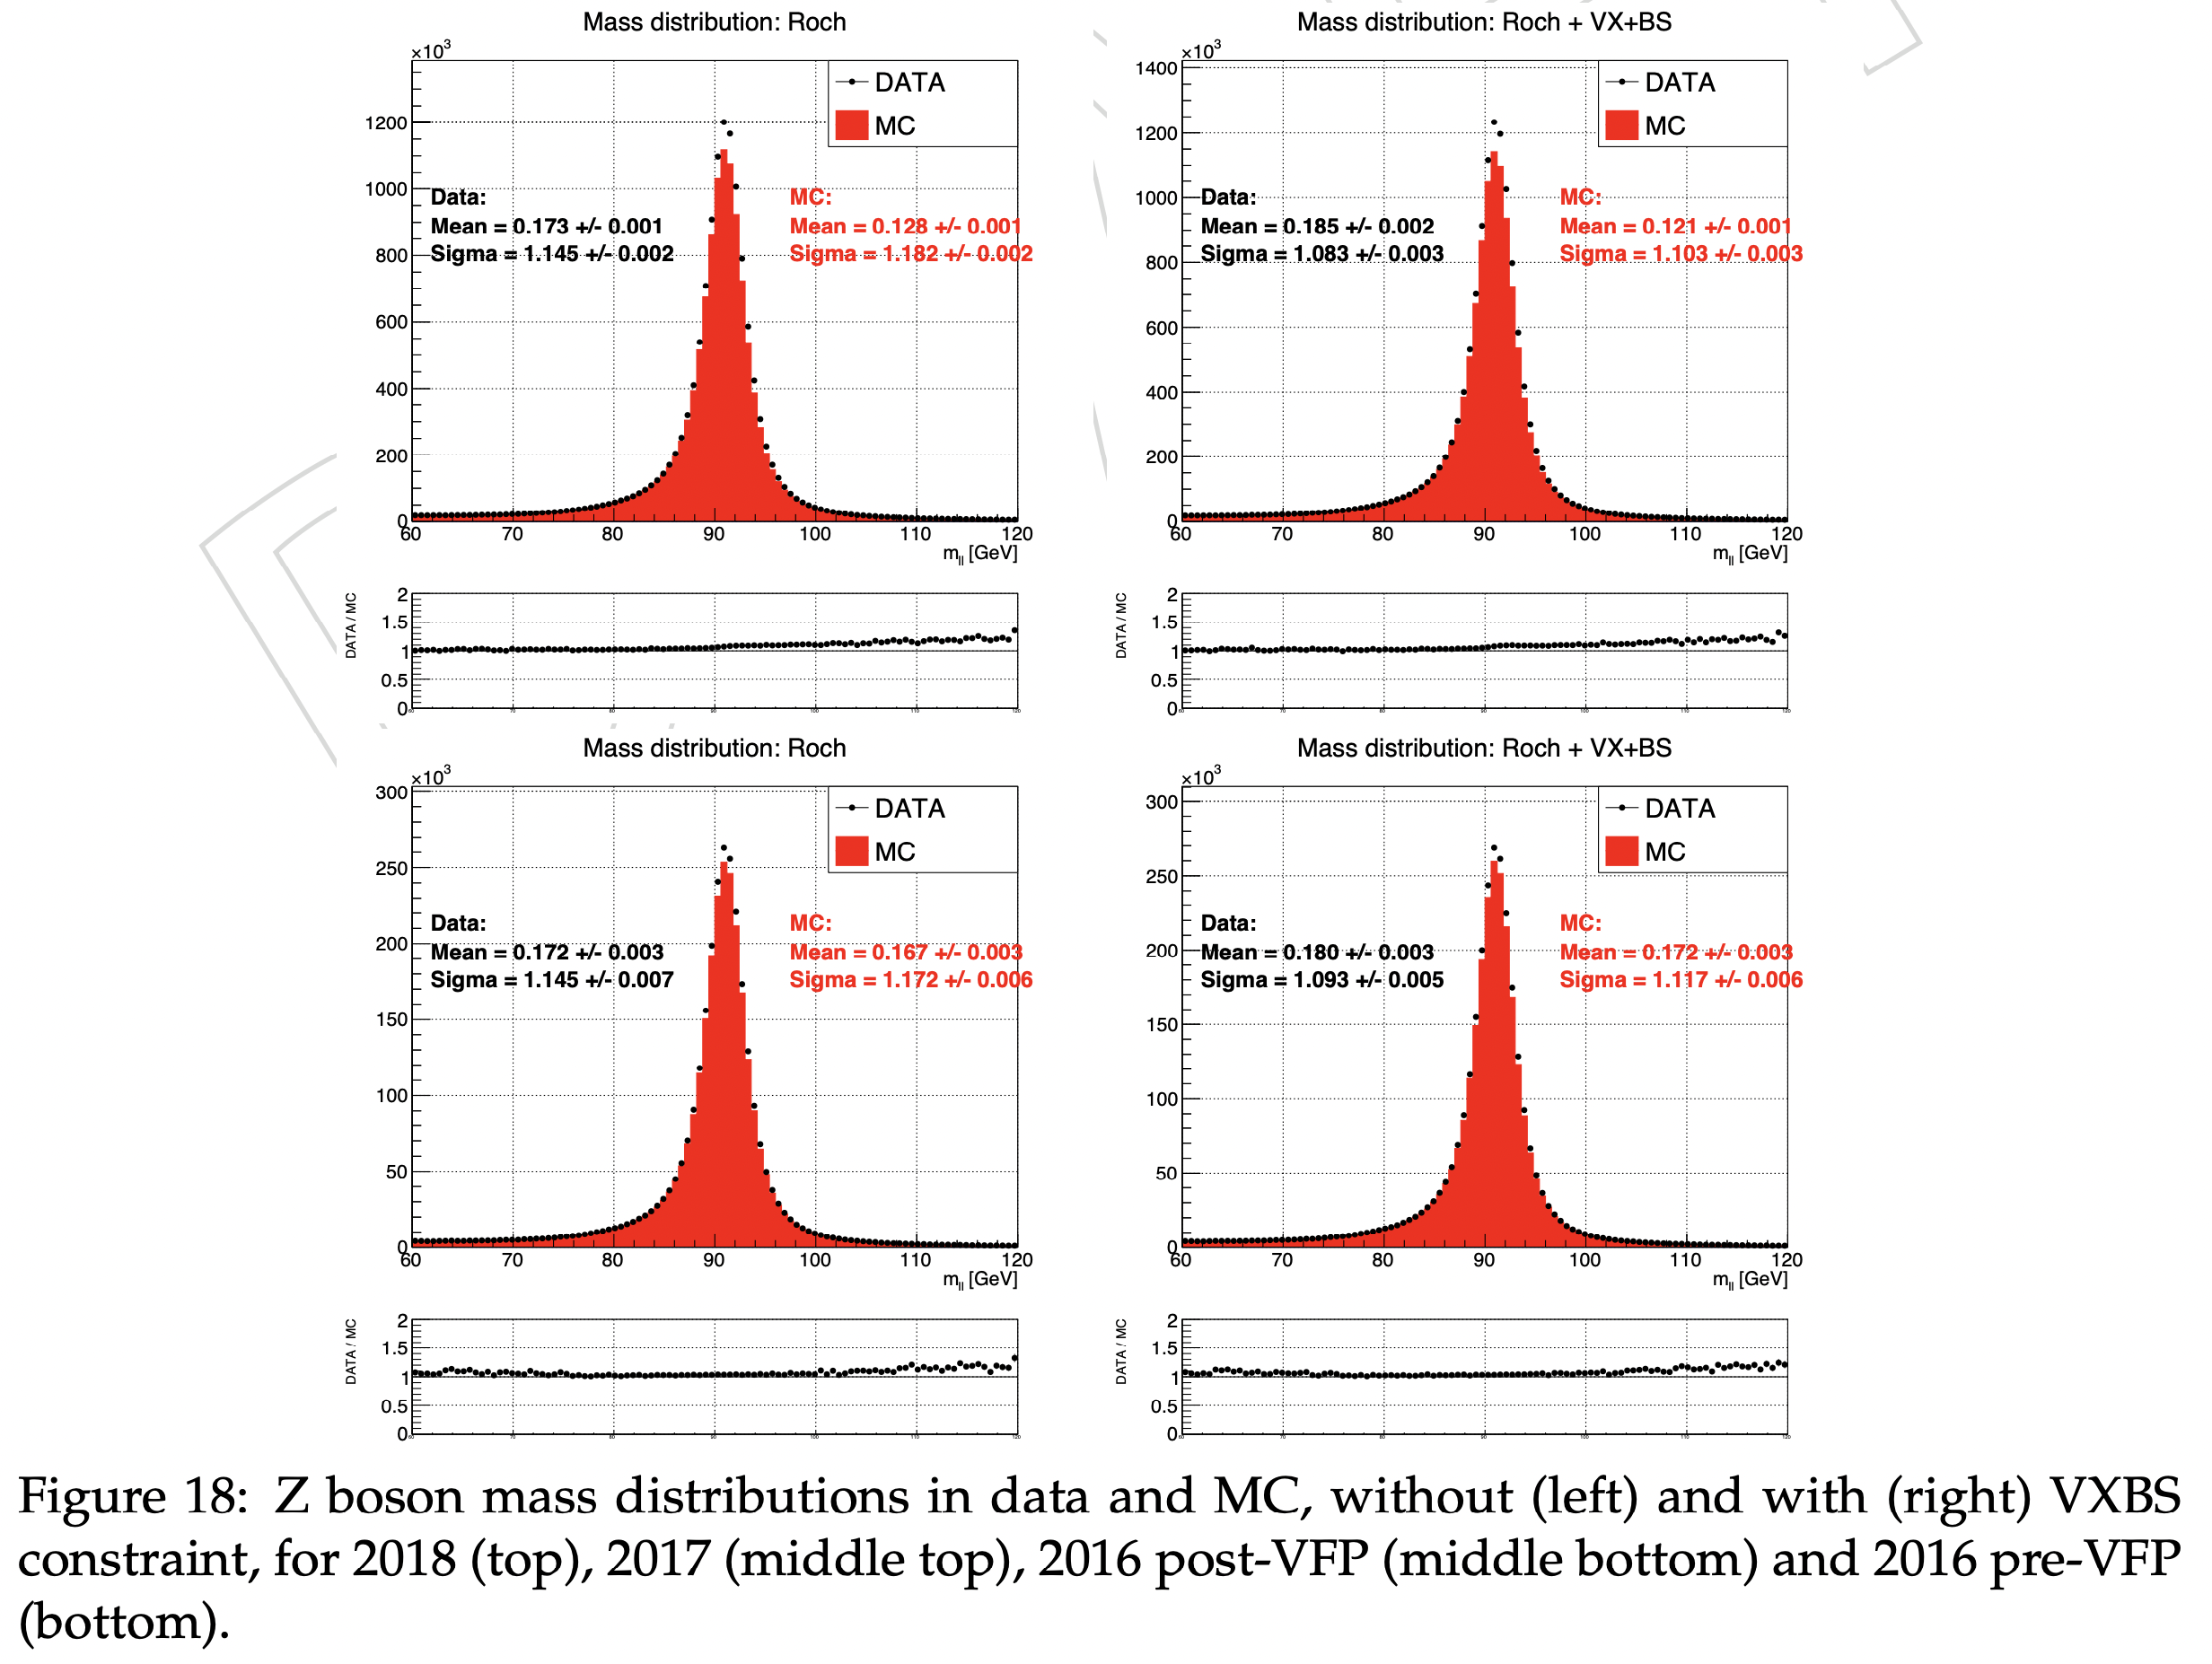
\includegraphics[width=0.96\textwidth]{figures/higgsmassmeas/vxbs/vxbs_mZdist_2016preVFP_2016postVFP.png}
    \captionof{figure}
        [\PZ boson mass distributions in data and MC, with and without VX+BS constraint]
        {\PZ boson mass distributions in data and MC, without (left) and with (right) VX+BS constraint. % TODO: REWORD 
        \;A) 2018.
        \;B) 2017.
        \;C) 2016 post-VFP.
        \;D) 2016 pre-VFP.} % TODO: Use actual PDFs. Split pic up properly?
\label{UL_ZBoson_DataMC_comparison_VXBS}
\end{multiFigure}

% More on beamspot constraint studies can be found in Appendix~\ref{app:adhoc_studies}. % TODO:Link not showing up % TODO: Fix appendix.

%=== 1D likelihood fit after VX+BS ===%
The updated invariant mass distributions, after applying the VX+BS constraint, are shown in Fig.~\ref{fig:1D_VXBS_mass_2018_ggH}.
\begin{multiFigure}
    \centering
        \addFigure{0.45}{figures/higgsmassmeas/ggH_MassDistribution/1D_VXBS_mass_2018_ggH_4mu.pdf}
        \addFigure{0.45}{figures/higgsmassmeas/ggH_MassDistribution/1D_VXBS_mass_2018_ggH_4e.pdf}
        \addFigure{0.45}{figures/higgsmassmeas/ggH_MassDistribution/1D_VXBS_mass_2018_ggH_2e2mu.pdf}
        \addFigure{0.45}{figures/higgsmassmeas/ggH_MassDistribution/1D_VXBS_mass_2018_ggH_2mu2e.pdf}
    \captionof{figure}
        [Four-lepton invariant mass distribution, after applying the VX+BS constraint]
        {Four-lepton invariant mass distribution, after applying the VX+BS constraint in the signal region ([105-140]\GeV) using ggH events, with the DSCB fit for 2018.
        \;A) 4$\mu$.    % TODO: fix symbols
        \;B) 4e.
        \;B) 2e2$\mu$.
        \;B) 2$\mu$2e.}
    \label{fig:1D_VXBS_mass_2018_ggH}
\end{multiFigure}
As can been seen, comparing these new distributions (Fig.~\ref{fig:1D_VXBS_mass_2018_ggH}, TODO) with the ones before beamspot constraint (Fig.~\ref{fig:1D_VXBS_mass_2018_ggH}, TODO), the $\sigma$ in 4$\mu$ final state has improved by 7$\%$, 4e is not affected (as expected), while mixed flavor final states show an improvement of a few percent.

\subsubsection{Expected \mH measurement uncertainties (MC)}
The expected $\mass{H}$ measurement uncertainties comparing VX+BS constraint to the baseline expectations can be seen in Table~\ref{table:1D_model_result_fs_BS} split by final state or in Table~\ref{table:1D_model_result_year_BS} split by year.

\begin{table}[ht]	
\begin{center}
    \topcaption
        [Expected Higgs boson mass uncertainty measured with 1D model, with and without VXBS, by final state]
        {Expected Higgs boson mass uncertainty measured with 1D model, with and without
        VX+BS for different final states. All mass values are given in \MeVns.
        Statistical-only results are considered at this stage of the analysis.
        }
    \begin{tabular}{ccccccc}
            \hline			
        Expected uncertainty (\MeVns)	&	4$\mu$	&	4e	&	2e2$\mu$	&2$\mu$2e	& inclusive	& Rel. Improvement \\
            \hline			
        1$D_{VXBS}$  (No bkg)	&	137	&	394	&	275	&	266	&	108 &	-4\%	\\
            1D	(No bkg) &	147	&	394	&	276	&	273	&	112	&	-	\\
        %	1$D_{VXBS}$  (No bkg)	&	144	&	466	&	313	&	291	&	116	&	-4\%	\\	
        %	1D	(No bkg) &	153	&	466	&	315	&	300	&	121 	&	- \\
            \hline
    \end{tabular}
    \label{table:1D_model_result_fs_BS}
\end{center}
\end{table}
\begin{table}[ht]	
\begin{center}
    \topcaption
        [Expected Higgs boson mass uncertainty measured with 1D model, with and without VXBS, by year]
        {Expected Higgs boson mass uncertainty measured with 1D model, with and without
        VX+BS for different years. All mass values are given in \MeVns.
        Statistical-only results are considered at this stage of the analysis.
        }
    \begin{tabular}{ccccc}
        \hline			
    Expected uncertainty (\MeVns)	&	2016 pre-VFP	&	2016 post-VFP	&	2017	&	2018	\\
        \hline			
        1$D_{VXBS}$	(No bkg)	&	291	&	301	&	198	&	162	\\
        1D (No bkg)	&	304	&	314	&	207	&	170	\\
    %	1$D_{VXBS}$	(No bkg)	&	227	&	212	&	173	\\
    %	1D (No bkg)	&	234	&	222	&	182	\\
        \hline
    \end{tabular}
    \label{table:1D_model_result_year_BS}
\end{center}
\end{table}
